Dans cette partie, nous nous plaçons dans une situation où deux forces gravitationnelles de coefficients 1 (resp. 0.01) centrées en $[0, 0]$ (resp. $[1, 0]$)

Une troisième force, centrifuge, de coefficient 1 et centrée sur le barycentre des deux précédentes. Ce point $(x, y)$ peut être trouvé en résolvant le système suivant :

$$
\begin{cases}
  a(A_x - x) + b(B_x - x) = 0 \\
  a(A_y - y) + b(B_y - y) = 0
\end{cases}
$$

avec $a$ et $(A_x, A_y)$ (resp. $b$ et $(B_x, B_y)$) respectivement le coefficient et le point d'application de la première (resp. deuxième) force gravitationnelle décrite précédemment.

Après résolution, on obtient $x = \frac{0,01}{1,01}$ et $y = 0$ comme coordonnées du point d'application de la force centrifuge.

\bigskip

Afin de calculer les points d'équilibre de ce système, nous allons utiliser plusieurs fois l'algorithme implémenté dans la partie \ref{sec:newton}. Après plusieurs itérations de l'algorithme en utilisant des points initiaux différents, on obtient cinq points d'équilibres : \emph{P1} = [0,5  0,870], \emph{P2} = [0,5  -0,870], \emph{P3} = [-0,998  0], \emph{P4} = [0,859  0], \emph{P5} = [1,158  0].

Ces points sont représentés sur la figure \ref{fig:equi_pts} :

\begin{figure}[ht]
  \centering
  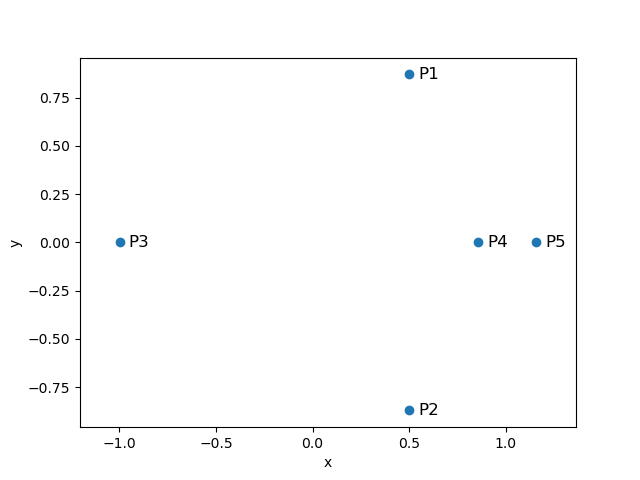
\includegraphics[width=0.5\textwidth]{img/equilibrium_points.png}
  \caption{Les différents points d'équilibre dans la plan de la situation décrite dans la partie \ref{ssec:lagrange}}
  \label{fig:equi_pts}
\end{figure}

\bigskip

Cette situation est celle d'une planète étant en orbite autour d'une étoile. Ici, la masse en position $[0, 0]$ est l'étoile, et celle en position $[1, 0]$ est la planète. Les points de Lagrange sont les points d'équilibre pour un objet de petite masse (par exemple un satellite) qui serait sous l'influence, dans notre cas, d'une étoile et d'une planète gravitant autour d'elle. Les points d'équilibre que nous avons calculer précédemment sont donc les points de Lagrange de ce cas-ci.

En modifiant les valeurs des coefficients et des points d'applications des forces, on obtient d'autres points d'équilibre : les points de Lagrange. Il est important de rappeler que leurs coordonnées ne sont pas les coordonnées exactes. Elles sont obtenues avec une précision de 0.01 dans notre cas.

\bigskip

Nous pouvons vérifier nos résultats en les comparant avec les points de Lagrange dans la situation où la Terre orbite autour du Soleil. Ces points sont donnés dans la figure \ref{fig:lagr_pts}. Ces points sont en concordance avec nos résultats présents en figure \ref{fig:equi_pts}.

\begin{figure}[ht]
  \centering
  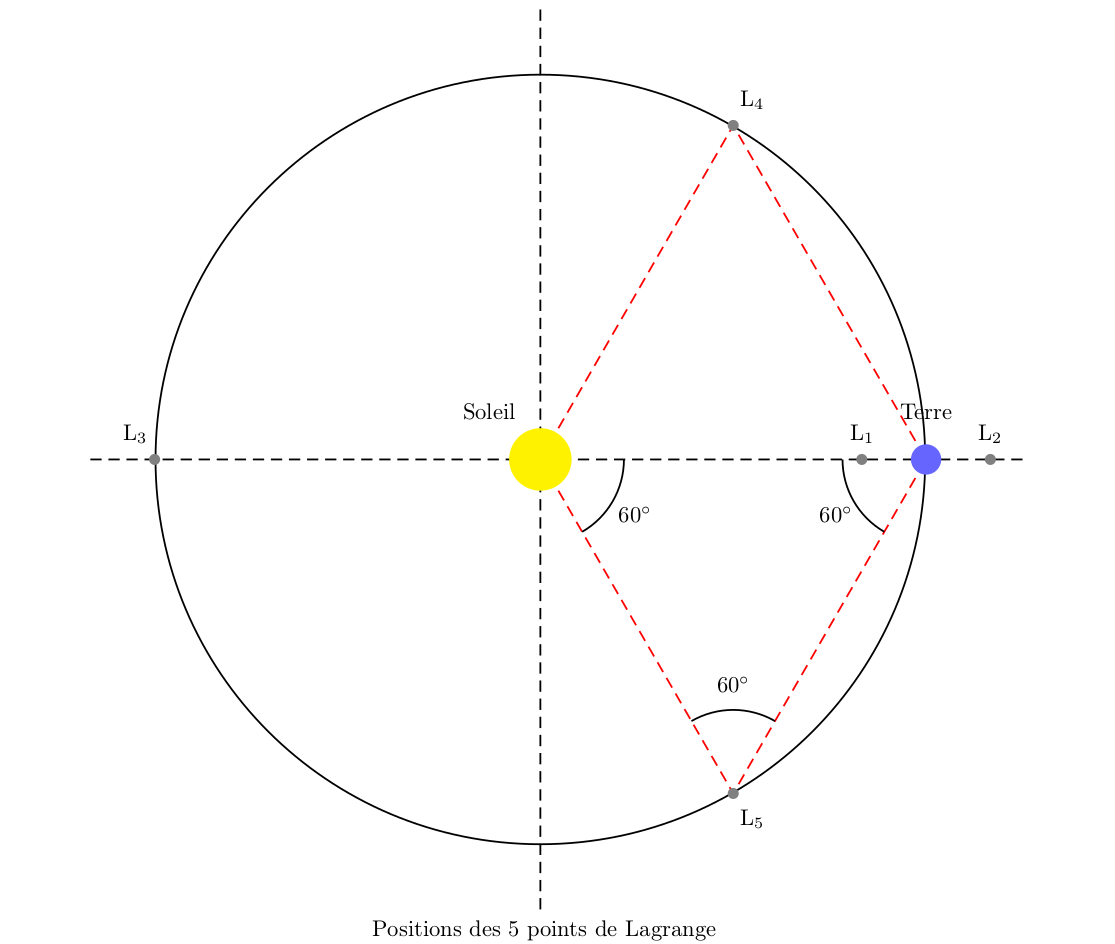
\includegraphics[width=0.5\textwidth]{img/lagrangian_points.png}
  \caption{Les points de Lagrange (L1...L5) dans le cas où la Terre orbite autour du Soleil}
  \label{fig:lagr_pts}
\end{figure}
